\section{Observador}

\begin{figure}[ht!]
\begin{center}
	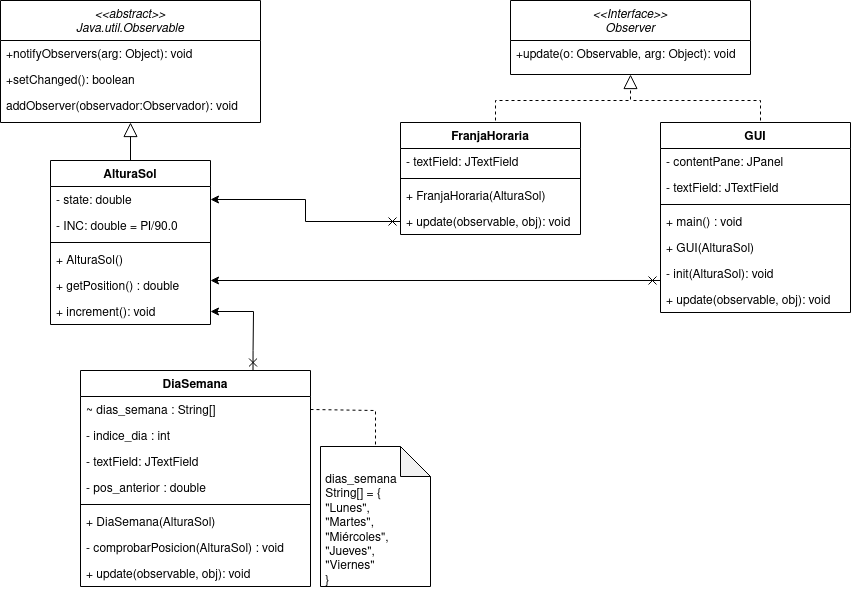
\includegraphics[scale=0.35]{DiagramaObservador}
\end{center}
\caption{Diagrama UML de la aplicación del patrón \textit{Observador}.}
\end{figure}

Para el patrón \textit{Observador} se ha implementado una funcionalidad básica pero imprescindible para \textit{CaveArt}: la altura del Sol y, consecuentemente, los días transcurridos y la franja horaria. Esto determina el paso del tiempo en la aplicación y el ciclo día-noche, necesarios para múltiples aspectos del juego, tales como:

\begin{itemize}
	\item Generación de entidades nocturnas-diurnas
	\item Nivel de luz
	\item Crecimiento de las plantas
\end{itemize}

La altura del Sol se define por una función seno que recibe incrementos de $\pi/90$. Alcanza su cénit cuando $f(x)=1$, de igual forma que en $f(x)=-1$ será medianoche.

Esta será nuestra variable Observable, que extiende la clase abstracta \textit{Observable} de \texttt{Java.util.Observer}.

\begin{figure}[ht!]
\begin{center}
	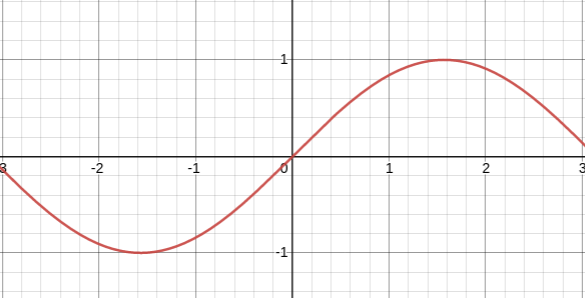
\includegraphics[scale=0.3]{Seno}
\end{center}
\caption{Función seno}
\end{figure}

El día de la semana se calcula en función al número de ciclos transcurridos, y se ejecuta concurrentemente a la hebra de \texttt{AlturaSol}.

Nuestro observador no suscrito es la franja horaria. Como ya hemos explicado, cuando la altura es menor que 0 se considerará que es de noche, y viceversa para el día.

Finalmente, la GUI se ha desarrollado en Eclipse mediante extensiones de JPanel. Es aquí donde se implementa el observador suscrito, que imprime constantemente la altura actual del Sol.
